
\subsubsection{Component Diagram}

Hệ thống được thiết kế theo kiến trúc hướng dịch vụ, đảm bảo tính đóng gói (Encapsulation) thông qua các giao diện (Interfaces) rõ ràng.

\begin{figure}[h]
    \centering
    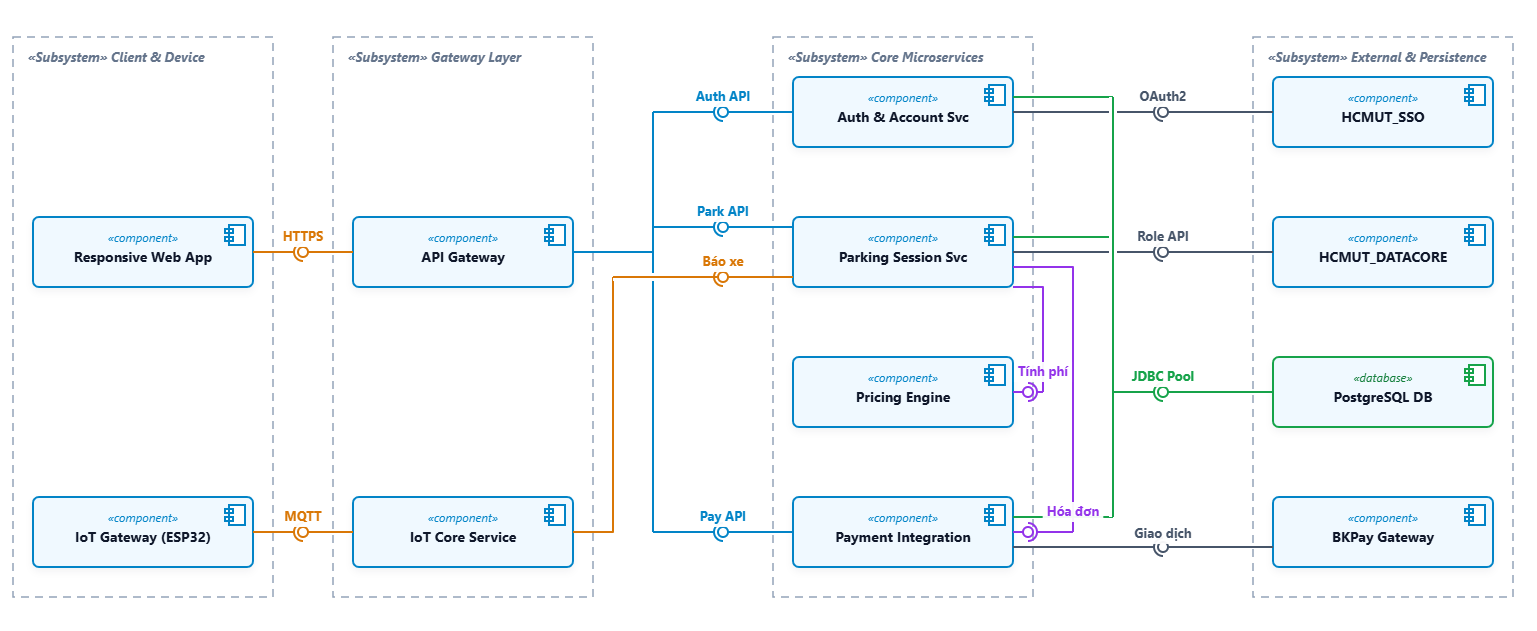
\includegraphics[width=0.75\linewidth]{pictures/component.png}
    \label{fig:placeholder}
\end{figure}

\subsection{Cấu trúc mã nguồn và Tổ chức Package}

Để đảm bảo tính bảo trì và khả năng mở rộng của hệ thống theo kiến trúc Microservices, mã nguồn được tổ chức dựa trên nguyên tắc thiết kế hướng miền (Domain-Driven Design - DDD). Cách tiếp cận này giúp tách biệt rõ ràng giữa logic nghiệp vụ, giao tiếp dữ liệu và cấu hình hạ tầng kỹ thuật.

\subsubsection{Cấu trúc Backend Core (Spring Boot / Node.js)}
Mã nguồn Backend được phân chia thành các package chức năng độc lập, giúp giảm thiểu sự phụ thuộc lẫn nhau (Low Coupling):
\begin{itemize}
    \item \texttt{com.iot\_spms.config}: Đóng vai trò là trung tâm cấu hình của hệ thống, quản lý các thiết lập về bảo mật (Security Context), cấu hình kết nối MQTT Broker và các tham số môi trường cho Database.
    \item \texttt{com.iot\_spms.modules.auth}: Chịu trách nhiệm thực hiện quy trình định danh; tích hợp chặt chẽ với \textbf{HCMUT\_SSO} để xác thực và đồng bộ thông tin người dùng từ hệ thống nhà trường.
    \item \texttt{com.iot\_spms.modules.parking}: Chứa logic nghiệp vụ cốt lõi về quản lý phiên gửi xe, điều phối trạng thái vị trí đỗ và xử lý dữ liệu từ cảm biến.
    \item \texttt{com.iot\_spms.modules.payment}: Chuyên biệt cho việc tính toán hóa đơn dựa trên chính sách giá và thực hiện giao tiếp với cổng \textbf{BKPay} thông qua các API thanh toán.
    \item \texttt{com.iot\_spms.modules.iot}: Lớp xử lý trung gian cho các luồng dữ liệu thời gian thực, quản lý các kết nối WebSocket và chuyển đổi dữ liệu từ giao thức MQTT sang logic nghiệp vụ nội bộ.
    \item \texttt{com.iot\_spms.shared}: Thư viện dùng chung chứa các đối tượng chuyển đổi dữ liệu (DTOs), các lớp Exception tùy chỉnh và các hàm tiện ích (Utilities) được sử dụng xuyên suốt các module.
\end{itemize}

\subsubsection{Cấu trúc Frontend (React)}
Phần giao diện được tổ chức theo kiến trúc Component-based hiện đại, giúp tối ưu hóa việc tái sử dụng mã nguồn:
\begin{itemize}
    \item \texttt{/src/components}: Chứa các UI components như  các bảng điều khiển và thành phần điều hướng.
    \item \texttt{/src/pages}: Tổ chức theo các luồng nghiệp vụ chính của người dùng như Dashboard quản lý, lịch sử giao dịch và Trang cá nhân.
    \item \texttt{/src/services}: Lớp trừu tượng hóa các lệnh gọi API (thông qua Axios), giúp tách biệt logic xử lý giao diện với logic giao tiếp mạng.
    \item \texttt{/src/store}: Trung tâm quản lý trạng thái toàn cục, đảm bảo dữ liệu (như trạng thái bãi đỗ) luôn nhất quán trên mọi màn hình.
\end{itemize}

\subsubsection{Quản lý phụ thuộc và Thư viện sử dụng}
.

\begin{table}[H]
\centering
\renewcommand{\arraystretch}{1.3}
\begin{tabularx}{\textwidth}{|l|l|X|}
\hline
\rowcolor[HTML]{EFEFEF} 
\textbf{Thành phần} & \textbf{Thư viện chính} & \textbf{Vai trò trong kiến trúc} \\ \hline
\textbf{Backend Core} & Spring Security & Triển khai giao thức OAuth2, JWT và cơ chế phân quyền (RBAC) cho nhân viên và khách hàng. \\ \cline{2-3} 
 & Spring Data JPA & Framework ORM mạnh mẽ giúp tương tác với PostgreSQL, tối ưu hóa hiệu năng truy vấn dữ liệu. \\ \cline{2-3} 
 & Eclipse Paho & Thư viện MQTT Client chuyên dụng để duy trì kết nối ổn định và tin cậy với các thiết bị IoT Gateway. \\ \hline
\textbf{Real-time Logic} & Socket.io & Cung cấp khả năng giao tiếp hai chiều thời gian thực, đảm bảo cập nhật trạng thái vị trí đỗ tức thời lên giao diện. \\ \hline
\textbf{Frontend} & Axios & Xử lý các yêu cầu HTTP/HTTPS tới API Gateway với cơ chế Interceptor để đính kèm Token bảo mật. \\ \cline{2-3} 
 & Tailwind CSS & Framework CSS hiện đại giúp xây dựng giao diện Responsive linh hoạt, đáp ứng tiêu chuẩn trải nghiệm người dùng (NFR4). \\ \hline
\textbf{IoT Gateway} & PubSubClient & Giao thức truyền tin gọn nhẹ (Lightweight), tối ưu cho các vi điều khiển có tài nguyên hạn chế. \\ \hline
\end{tabularx}
\caption{Bảng tổng hợp các thư viện và công nghệ then chốt trong hệ thống IoT-SPMS.}
\end{table}




